\section{Modelli per l'Object Detection}

Nel campo dell'Object Detection, vari modelli hanno rivoluzionato il rilevamento degli oggetti nelle immagini, contribuendo significativamente alla precisione e all'efficienza di questa tecnologia fondamentale della Computer Vision. Ogni modello presenta un approccio distintivo per affrontare le sfide di localizzazione e classificazione degli oggetti.

\subsection{R-CNN e Varianti}

\subsubsection{R-CNN}
R-CNN (Region-based Convolutional Neural Network) è stato uno dei primi modelli ad adottare un approccio basato sulle region proposals per l'Object Detection. Proposto da Ross Girshick, Jeff Donahue, Trevor Darrell e Jitendra Malik nel 2014 \cite{6}, ha segnato un punto di svolta nell'utilizzo delle reti neurali convoluzionali per il rilevamento degli oggetti. Prima dell'introduzione di R-CNN, i metodi tradizionali per l'Object Detection erano basati su tecniche di estrazione di features manuali e classificatori separati. Questi approcci erano spesso limitati dalla necessità di progettare manualmente le features e dalla loro mancanza di robustezza e generalizzazione.

R-CNN si distingue per il suo approccio in tre fasi visto precedentemente:

\begin{enumerate}
    \item \textbf{Generazione delle Proposal Regions}: genera un insieme di proposal regions candidate tramite algoritmi come il Selective Search, le quali vengono poi selezionate in base a caratteristiche di basso livello come colore, texture e forma.
    \item \textbf{Feature Extraction}: ogni proposal region viene trasformata in una dimensione fissa e passata attraverso una rete convoluzionale pre-addestrata, come AlexNet o VGG-16. Questo processo genera una feature map per ciascuna region proposal, catturando le informazioni rilevanti dell'area proposta.
    \item \textbf{Classificazione e Ottimizzazione delle Bounding Box}: le feature estratte da ciascuna region proposal vengono fornite a un classificatore SVM per determinare la presenza di oggetti e per la classificazione, mentre un regressore lineare ottimizza le coordinate della bounding box prevista per migliorare la precisione della localizzazione dell'oggetto.
\end{enumerate}

\begin{figure}[ht]
    \centering
    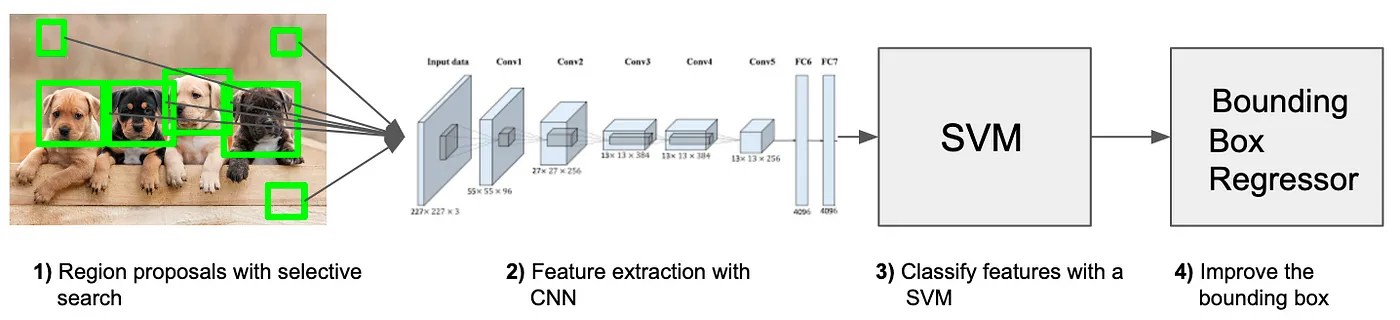
\includegraphics[width=1\textwidth]{files/capitoli/1-object-detection/assets/r-cnn.png}
    \caption{\label{fig:r-cnn}Architettura di R-CNN\cite{7}}
\end{figure}

\vspace{1.7cm}

\subsubsection{Fast R-CNN}
Fast R-CNN, proposto da Ross Girshick nel 2015\cite{8}, migliora l'efficienza di R-CNN introducendo le seguenti migliorie:

\begin{itemize}
    \item \textbf{Utilizzo di una sola CNN}: integra l'intero processo di rilevamento degli oggetti in una singola rete, combinando l'estrazione di features e la generazione di region proposals
    \item \textbf{RoI Pooling}: introduce la tecnica di RoI (Region of Interest) pooling per estrarre features dalle feature map generate, gestendo efficacemente regioni di dimensioni variabili.
\end{itemize}

\begin{figure}[ht]
    \centering
    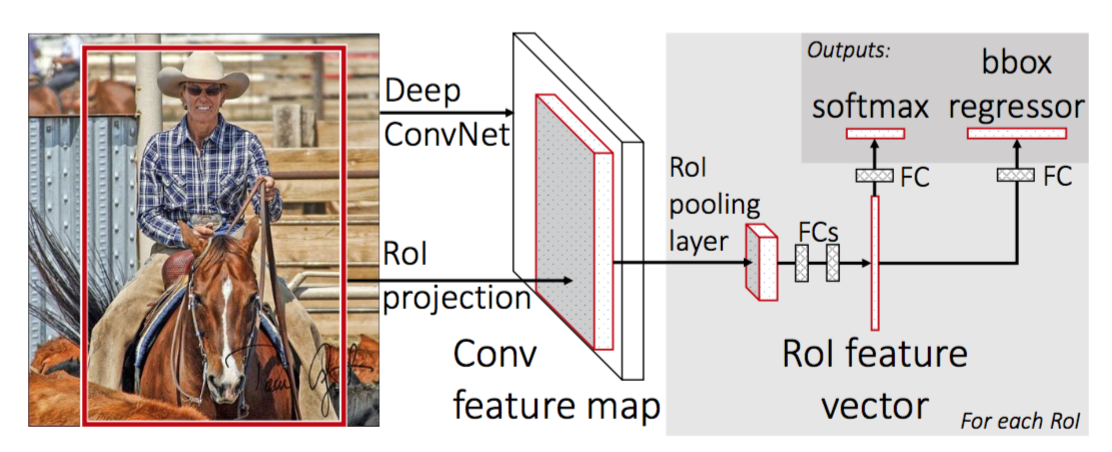
\includegraphics[width=0.8\textwidth]{files/capitoli/1-object-detection/assets/fast-r-cnn.png}
    \caption{\label{fig:fast-r-cnn}Architettura di Fast R-CNN\cite{9}}
\end{figure}

\vspace{1.6cm}

\subsubsection{Faster R-CNN}
Faster R-CNN, proposto da Shaoqing Ren, Kaiming He, Ross Girshick e Jian Sun nel 2016\cite{10}, rappresenta un ulteriore miglioramento rispetto a Fast R-CNN, introducendo un approccio più efficiente per la generazione delle region proposals. Principali migliorie: 

\begin{itemize}
    \item \textbf{Region Proposal Network (RPN)}: introduce una RPN che opera condividendo la feature map con la rete principale, permettendo la generazione di proposte di regioni in modo efficiente e integrato.
    \item \textbf{Architettura two-stage}: divide il processo di rilevamento degli oggetti in due fasi: prima, il RPN propone regioni d'interesse basate sulla feature map condivisa; successivamente, queste proposte vengono elaborate da un classificatore e un regressore per la classificazione degli oggetti e l'ottimizzazione delle bounding box.
    \item \textbf{RoI Pooling migliorato}: implementa un RoI pooling migliorato all'interno dell'RPN e nella fase successiva di elaborazione delle proposte. Questo approccio ottimizza la gestione delle regioni di interesse, migliorando la precisione complessiva del rilevamento degli oggetti.
\end{itemize}

\begin{figure}[ht]
    \centering
    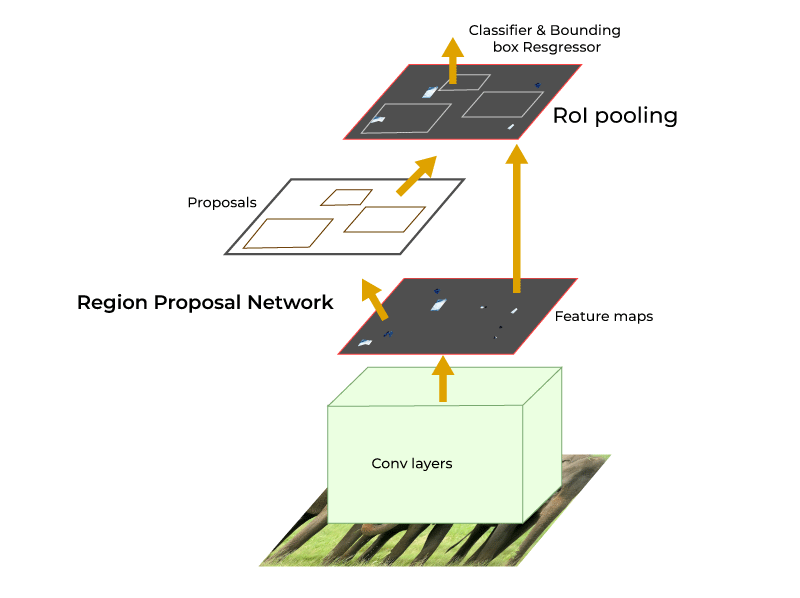
\includegraphics[width=0.8\textwidth]{files/capitoli/1-object-detection/assets/faster-r-cnn.png}
    \caption{\label{fig:faster-r-cnn}Architettura di Faster R-CNN\cite{9}}
\end{figure}

\newpage

\subsection{SSD}
Il modello SSD (Single Shot MultiBox Detector) è stato un importante avanzamento nell'ambito dell'Object Detection. Proposto da Wei Liu, Dragomir Anguelov, Dumitru Erhan, Christian Szegedy, Scott Reed, Cheng-Yang Fu e Alexander C. Berg nel 2016\cite{11}, ha introdotto un approccio single-shot per il rilevamento degli oggetti, combinando predizione delle bounding box e classificazione degli oggetti in un unico passaggio. Prima dell'SSD, i modelli two-stage come R-CNN e le sue varianti dominavano il campo, con una fase separata di generazione delle region proposals seguita dalla classificazione. Questi approcci, sebbene accurati, erano spesso limitati dalla complessità computazionale e dalla lentezza del processo.
Eliminando questa fase separata adottata dai modelli two-stage, rende il processo di rilevamento più rapido ed efficiente. Questa caratteristica ha reso SSD ideale per applicazioni che richiedono un'elaborazione veloce delle immagini, come la videosorveglianza e i sistemi di guida autonoma.

\begin{figure}[ht]
    \centering
    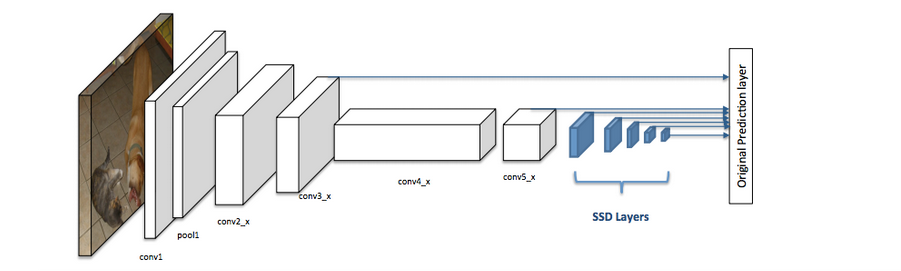
\includegraphics[width=0.95\textwidth]{files/capitoli/1-object-detection/assets/ssd.png}
    \caption{\label{fig:ssd}Architettura di SSD\cite{12}}
\end{figure}

Un'altra innovazione chiave di SSD è l'utilizzo delle \textbf{anchor box}: bounding box con dimensioni predefinite disposte su una griglia che suddivide l'immagine. Durante l'addestramento, SSD predice l'offset rispetto a ciascuna anchor box per adattare la posizione e le dimensioni della bounding box alle caratteristiche specifiche dell'oggetto da rilevare.

Questo approccio consente a SSD di individuare oggetti di diverse dimensioni e forme con maggiore accuratezza e robustezza.

\begin{figure}[ht]
    \centering
    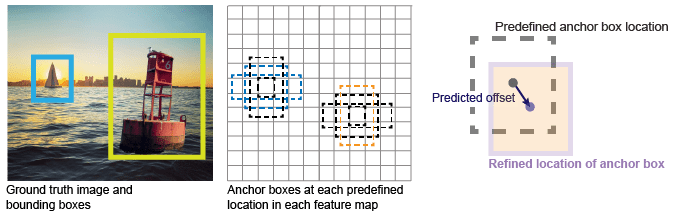
\includegraphics[width=1\textwidth]{files/capitoli/1-object-detection/assets/ssd-anchors.png}
    \caption{\label{fig:ssd-anchors}Utilizzo delle anchor box nell'SSD\cite{13}}
\end{figure}

SSD rappresenta quindi un passo significativo verso modelli più efficienti e versatili per l'Object Detection, combinando alta precisione con prestazioni ottimali in tempo reale.

\subsection{YOLO}
Il modello YOLO (You Only Look Once) rappresenta un'altra pietra miliare nell'ambito dell'Object Detection, affiancandosi all'SSD come uno dei primi modelli single-shot a rivoluzionare il campo. Proposto originariamente da Joseph Redmon, Santosh Divvala, Ross Girshick e Ali Farhadi nel 2016\cite{14}, YOLO segue l'approccio innovativo che combina la predizione delle bounding box e la classificazione degli oggetti in un singolo passaggio. Come nell'SSD, l'immagine viene suddivisa in una griglia e vengono predette bounding box e probabilità di classe direttamente per ciascuna cella della griglia.

YOLO si distingue per la sua capacità di considerare il contesto globale dell'immagine durante il processo di rilevamento. Ogni cella della griglia non solo predice le bounding box ma valuta anche la confidenza di ciascuna predizione in relazione a tutte le altre predizioni nell'immagine. Questo approccio globale contribuisce a migliorare la coerenza e la precisione complessiva del modello.

Inoltre, YOLO utilizza un'unica CNN per l'intero processo di rilevamento degli oggetti, semplificando ulteriormente l'architettura e migliorando l'efficienza computazionale. Questa caratteristica lo rende particolarmente adatto per dispositivi con risorse limitate e per applicazioni embedded.

\begin{figure}[ht]
    \centering
    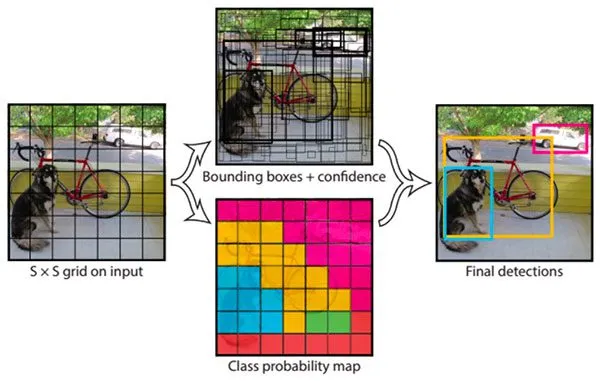
\includegraphics[width=0.8\textwidth]{files/capitoli/1-object-detection/assets/yolo.png}
    \caption{\label{fig:yolo}Object Detection tramite YOLO\cite{15}}
\end{figure}

YOLO ha trovato ampio impiego in una vasta gamma di applicazioni, dalla videosorveglianza alla guida autonoma, grazie alla sua velocità, precisione e capacità di gestire oggetti di diverse dimensioni e forme all'interno di un'immagine.

\newpage

